% Schematic of the polariton

\tikzset{every picture/.style={line width=0.75pt}} %set default line width to 0.75pt

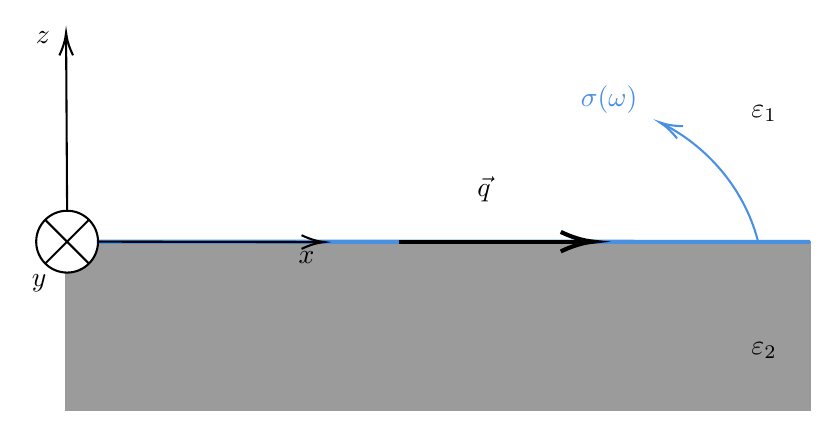
\begin{tikzpicture}[x=0.75pt,y=0.75pt,yscale=-1,xscale=1]
%uncomment if require: \path (0,260); %set diagram left start at 0, and has height of 260

%Shape: Rectangle [id:dp06901463979745426]
    \draw  [color={rgb, 255:red, 155; green, 155; blue, 155 }  ,draw opacity=1 ][fill={rgb, 255:red, 155; green, 155; blue, 155 }  ,fill opacity=1 ] (40.9,128.6) -- (399.47,128.6) -- (399.47,209.5) -- (40.9,209.5) -- cycle ;
%Straight Lines [id:da06539523190990693]
    \draw    (41.5,113.6) -- (41.01,29.8) ;
    \draw [shift={(41,27.8)}, rotate = 89.67] [color={rgb, 255:red, 0; green, 0; blue, 0 }  ][line width=0.75]    (10.93,-3.29) .. controls (6.95,-1.4) and (3.31,-0.3) .. (0,0) .. controls (3.31,0.3) and (6.95,1.4) .. (10.93,3.29)   ;
%Straight Lines [id:da9733818733234405]
    \draw [color={rgb, 255:red, 74; green, 144; blue, 226 }  ,draw opacity=1 ][line width=1.5]    (41.5,128.5) -- (399.47,128.6) ;
%Straight Lines [id:da6276402814533844]
    \draw    (56.4,128.5) -- (163.4,128.7) ;
    \draw [shift={(165.4,128.7)}, rotate = 180.11] [color={rgb, 255:red, 0; green, 0; blue, 0 }  ][line width=0.75]    (10.93,-3.29) .. controls (6.95,-1.4) and (3.31,-0.3) .. (0,0) .. controls (3.31,0.3) and (6.95,1.4) .. (10.93,3.29)   ;
%Straight Lines [id:da79763264474433]
    \draw [color={rgb, 255:red, 0; green, 0; blue, 0 }  ,draw opacity=1 ][line width=1.5]    (201.17,128.5) -- (291.97,128.5) ;
    \draw [shift={(294.97,128.5)}, rotate = 180] [color={rgb, 255:red, 0; green, 0; blue, 0 }  ,draw opacity=1 ][line width=1.5]    (15.63,-4.7) .. controls (9.94,-1.99) and (4.73,-0.43) .. (0,0) .. controls (4.73,0.43) and (9.94,1.99) .. (15.63,4.7)   ;
%Flowchart: Summing Junction [id:dp10376160873516338]
    \draw  [fill={rgb, 255:red, 255; green, 255; blue, 255 }  ,fill opacity=1 ] (26.6,128.5) .. controls (26.6,120.27) and (33.27,113.6) .. (41.5,113.6) .. controls (49.73,113.6) and (56.4,120.27) .. (56.4,128.5) .. controls (56.4,136.73) and (49.73,143.4) .. (41.5,143.4) .. controls (33.27,143.4) and (26.6,136.73) .. (26.6,128.5) -- cycle ; \draw   (30.96,117.96) -- (52.04,139.04) ; \draw   (52.04,117.96) -- (30.96,139.04) ;
%Curve Lines [id:da5726507027737717]
    \draw [color={rgb, 255:red, 74; green, 144; blue, 226 }  ,draw opacity=1 ]   (374.67,129.5) .. controls (368.65,104.64) and (351.39,83.58) .. (328.75,71.88) ;
    \draw [shift={(327,71)}, rotate = 26.08] [color={rgb, 255:red, 74; green, 144; blue, 226 }  ,draw opacity=1 ][line width=0.75]    (10.93,-3.29) .. controls (6.95,-1.4) and (3.31,-0.3) .. (0,0) .. controls (3.31,0.3) and (6.95,1.4) .. (10.93,3.29)   ;

% Text Node
    \draw (151.5,132.0) node [anchor=north west][inner sep=0.75pt]    {$x$};
% Text Node
    \draw (23,142.9) node [anchor=north west][inner sep=0.75pt]    {$y$};
% Text Node
    \draw (25,25.9) node [anchor=north west][inner sep=0.75pt]    {$z$};
% Text Node
    \draw (237.67,95.9) node [anchor=north west][inner sep=0.75pt]  [color={rgb, 255:red, 0; green, 0; blue, 0 }  ,opacity=1 ]  {$\vec{q}$};
% Text Node
    \draw (366.67,58.4) node [anchor=north west][inner sep=0.75pt]    {$\textcolor[rgb]{1,1,1}{\varepsilon }\textcolor[rgb]{1,1,1}{_{1}}$};
% Text Node
    \draw (369.67,175.4) node [anchor=north west][inner sep=0.75pt]  [color={rgb, 255:red, 0; green, 0; blue, 0 }  ,opacity=1 ]  {$\varepsilon _{2}$};
% Text Node
    \draw (369.67,61.4) node [anchor=north west][inner sep=0.75pt]  [color={rgb, 255:red, 0; green, 0; blue, 0 }  ,opacity=1 ]  {$\varepsilon _{1}$};
% Text Node
    \draw (287.5,51.9) node [anchor=north west][inner sep=0.75pt]    {$\textcolor[rgb]{0.29,0.56,0.89}{\sigma ( \omega )}$};


\end{tikzpicture}
